% This file should be replaced with your file with an thesis content.
%=========================================================================
% Authors: Michal Bidlo, Bohuslav Křena, Jaroslav Dytrych, Petr Veigend and Adam Herout 2019

\definecolor{darkpastelred}{rgb}{0.76, 0.23, 0.13}
\definecolor{codegreen}{rgb}{0,0.6,0}
\definecolor{codegray}{rgb}{0.5,0.5,0.5}
\definecolor{codepurple}{rgb}{0.58,0,0.82}
\definecolor{backcolour}{rgb}{0.95,0.95,0.92}
\lstset{
    string=[s]{"}{"},
    stringstyle=\color{darkpastelred},
    comment=[l]{:},
    commentstyle=\color{black},
    caption=Example of event described using CloudEvents specification and JSON
}


\lstdefinestyle{jsonStyle}{
    string=[s]{"}{"},
    stringstyle=\color{darkpastelred},
    comment=[l]{:},
    breaklines=true,
    commentstyle=\color{black}
}

\lstdefinestyle{pythonStyle}{
    backgroundcolor=\color{backcolour},
    commentstyle=\color{codegreen},
    keywordstyle=\color{blue},
    numberstyle=\tiny\color{codegray},
    stringstyle=\color{codepurple},
    basicstyle=\ttfamily\footnotesize,
    breakatwhitespace=false,
    breaklines=true,
    captionpos=b,
    keepspaces=true,
    numbers=left,
    showspaces=false,
    showstringspaces=false,
    showtabs=false,
    tabsize=2
}

\hyphenation{OpenStack Swift OpenIO SDS}

\chapter{Introduction}\label{chap:introduction}

% general introduction for a topic:
%- cloud computing popularity
%- most popular service: cloud storage and its types
%- about object storage
%- users interest of what's going in theirs storage / event activities
%- TODO: maybe remove talk about types of cloud storages? solution: talk about need for monitoring and users need to monitor/receive information regarding their storage
In the current world, cloud computing has become the most popular way of delivering different services on the Internet. One of the most popular cloud services is cloud storage, allowing users to store data in remote locations maintained by a third party. Based on how cloud storage manages data, cloud storage can be divided into three types: Block storage, File storage and Object storage. Object storage manages data as objects, and each object typically includes data itself and some additional information stored in objects metadata. Since data are stored in remote locations, to which users do not have direct and complete access, some users or external services might want to receive information about specific events (for example, change of content) in storages where their data are located.

% importance of thesis in this field
%- react to events - possibly react to 'bad' events
%- allows users to have a better picture of what is going on in their storage
The importance of this thesis is to provide event information to users in OpenIO SDS and OpenStack Swift, which will allow users to react to those events, create more sophisticated backend operations and postprocessing, or possibly prevent/detect unwanted actions. In addition, providing event notifications will allow users to have a better picture of what is going on in their storage and improve monitoring in these object storages.

%past advances in this field
There were two attempts\cite{swiftPatch1}\cite{swiftPatch2} to solve this issue within OpenStack Swift which were not officially accepted, and their solution is outdated. So currently, there is no official solution for publishing event notification in OpenStack Swift nor OpenIO Software-Defined Storage (from now on SDS).

%why am I interested in this, why I choose this topic
%- perosnally i used object storage
%- can se myself using this solution in future as well as millions of other users
%- impact on big amount of users
%- contibuting to open source projects
My interest in this topic stems from its possible impact on the extensive amount of users that OpenStack Swift and OpenIO have. Furthermore, I have always wanted to contribute to open-source projects. The possibility to improve user experience in OpenStack Swift and OpenIO SDS and allow these storages to be even more competitive against commercial storages (Amazon, Google, ...) is another reason why I choose this topic.

%goals of thesis
This thesis aims to create a program/middleware which will publish event notifications to user-specified destinations. One of the supported destinations will be the Beanstalk queue, but the program can be easily configured to support other destinations (for example, Kafka) using a predefined interface. The proposed program will allow users to specify, using objects metadata (such as name prefix/suffix and object size) and type of event, which event notification should be published. The program will be able to run within OpenStack Swift and OpenIO SDS. This thesis will strive to find such a solution that could be officially accepted as part of OpenStack Swift and OpenIO SDS.

%structure of thesis
This work consists of six chapters. Chapter \ref{chap:introduction} introduces the motivation, objectives, and proposed solutions of this work. Chapter \ref{chap:background} briefly describes technologies and general areas that this work relates to. Chapter \ref{chap:openiosds} covers OpenIO SDS, describes its data organization and key services providing events. Chapter \ref{chap:swift} introduces OpenStack object storage Swift, its data model, server processes and describes middlewares within OpenStack Swift. Chapter \ref{chap:minio} briefly covers MinIO storage and the way it publishes event notifications. Chapter \ref{chap:solution} describes the current state of event notifications in OpenIO SDS, OpenStack Swift and MinIO, and proposes a solution for publishing event notifications in OpenIO SDS and OpenStack, and a solution for publishing event notifications from MinIO to Beanstalk queue.

Chapters \ref{chap:openiosds}, \ref{chap:swift}, and \ref{chap:minio} deal with the first point of the assingment, while chapter \ref{chap:solution} deals with the second point of assigment.



\chapter{Background}\label{chap:background}

    This chapter introduces Object storage, its core concepts, and the underlying technologies. After introducing the Object storage, for sufficient understanding of this master thesis topic, it is essential to explain how Software-defined storage manages data and what types of events can occur inside. The last part of this chapter describes the concept of event notifications, why they are essential, and current interfaces for publishing them to users.

\section{Object storage}
    %introduction/concept
    Object storage, also known as \textit{object-based storage (OBS)}, handles data as objects instead of hierarchical methods used in file systems\cite{objectBasedStorage}. The object storage is designed to handle data as whole objects, making it an ideal solution for any unchanging data. Data in object stores are changed by replacing objects or files, and therefore object stores are the preferred mechanism for storing such files\cite{networkStorage}.

    %key koncepts
    %-metadata are stored in same object store device but on separated location
    \subsection*{Key concepts}
    Key concepts of object storage are\cite{ibmObjectStorage}:
    \begin{itemize}
        \item \textbf{Objects} - An object typically consist of user data and metadata uploaded to object storage.
        \item \textbf{Containers/Buckets} - represents logical abstraction used to provide a data container in object storage. An object with the same name in two different containers represents two different objects. This concept segregates data using bucket ownership and a combination of public and secret keys bound to object storage accounts, allowing users and applications to manipulate with authorized data for specific types of manipulation (read/write/update).
        \item \textbf{Metadata} - Additional information about data, such as date of creation and last modification, size, hash.
        \item \textbf{Access Control Lists(ACLs)} - used as primary security construct in object storage, stored in account or bucket level and allows owners to grant permissions for certain operations based on UUID, email, ...
        \item \textbf{Object Data protection} - two primary data protection schemes in object storage are Replication and Erasure Coding.

        \textbf{Replication} is a method used to ensure data resilience. Data are copied into multiple locations/disks/partitions. In case of failure, data are used from a secondary copy to recreate the original copy or as a primary copy.

        \textbf{Erasure coding} is a process through which the data is separated into fragments. Then fragments are expanded and encoded with redundant pieces and stored across different storage devices. Erasure coding adds redundancy and allows object storage to tolerate failures.
    \end{itemize}


    \subsection*{Object data}
    %types of stored informations
    With object storage techniques, each object contains\cite{ibmObjectStorage}:
    \begin{itemize}
      \item \textbf{Data} - user-specified data that needs to be stored in persistent storage. Such data can be binary data, text file, image, etc.
      \item \textbf{Metadata} - additional data that describe objects data. Metadata can be divided into two types: \textit{Device-managed metadata} is additional information maintained by a storage device and used as part of object management in physical storage\cite{objectBasedStorage}. The second type is \textit{Custom metadata}, to which users can store any additional information in key and value pairs. In object storage, metadata is stored together with the object.
      \item \textbf{A universally unique identifier (UUID)} - This ID, created using a hashing process based on object name and other additional information, is assigned to each object in object storage. Using ID object storage systems can tell apart objects from one another. ID is also used to extract data in a system without knowing their physical location/drive and offset.
    \end{itemize}

    \subsection*{Access to object storage}
    %access to object storage
    %-resfull interface
    %-advantages of this approach
    %-popular intefaces
    Object storage services provide a \texttt{RESTful} interface \cite{cloudObjectStorage} over \texttt{HTTP} protocol to store and access objects. This approach allows users to create, read, delete, update, or even query objects anytime and anywhere simply by referencing UUID (or using specific attributes for querying), usually with a proper authentication process. The most popular interfaces for communicating with object storages are \textit{Amazon S3 (Simple Storage Service) API} and \textit{OpenStack Swift API}.

    %comparison to other storage models
    \subsection*{Pros and cons of object storage}
    Pros:
    \begin{itemize}
        \item Capable of handling a large amount of unstructured data
        \item Reduced TCO and cheap COTS - Object storage is designed to utilize cheap COTS(Commercial off-the-shelf) components. As a result Total Cost of Ownership(TCO) is lower than owning homemade Network-Attached Storage(NAS)\cite{networkStorage}.
        \item Unlimited scalability - Since object storages are built on distributed systems, they scale very well compared to traditional storages, where they often have an upper limit\cite{swiftEssentials}.
        \item Wide-open metadata - allows users to store custom metadata and the possibility of creating metadata-driven policies, such as compression and tiering.
    \end{itemize}
    Cons:
    \begin{itemize}
        \item No in-place update - object must be manipulated as a whole unit.
        \item No locking mechanism - object storage does not manage object-level locking, and it is up to applications to solve concurrent PUT/GET.
        \item Slower - this makes object storages a poor choice for applications that need rapid and frequent access to data.
    \end{itemize}

\section{Software-Defined storage}
    %introduction to topic
    \textit{Software-Defined Storage(SDS)} is a storage architecture that separates software storage from hardware allowing greater scalability, flexibility, and control over the data storage infrastructure. With the growth of \textit{Software-Defined Networks(SDN)} and the need for \textit{Software-Defined Infrastructure(SDI)}, which aims to virtualize network resources and separate the control plane from the data plane, this principle was needed to be applied on Object storage as well\cite{sdsSDSMultiTenantEnv}.

    To overcome limitations of traditional storage infrastructures, the Software-Defined Storage is imposed as a proper solution to simplify data and configuration management while improving the end-to-end control functionality of conventional storage systems\cite{sdsSurvey}. Furthermore, while traditional storages like storage area networks (SAN) and network-attached storage (NAS) provides scalability and reliability, SDS provides it with much lower cost by utilizing industry-standard or x86 system and therefore removing dependency on expensive hardware\cite{sdsWPRedHatSDS}.

    %principles
    % - Scale-out
    % - Customizable
    % - Automation
    % - Masking
    % - Policy Management
    \subsection*{Principles}
    There is no clear definition on criteria for defining software-defined storage, although several fundamental principles can be deducted\cite{sdsGPCloudStorage}:
    \begin{itemize}
        \item \textbf{Scale-out} - SDS should enable low-cost horizontal scaling (by adding new commodity hardware to existing infrastructure) compared to vertical scaling with more powerful (and expensive) hardware.
        \item \textbf{Customizable} - SDS should offer system storage customization to meet specific storage QoS requirements. This will allow users to choose storage solution based on their requirements/performance and avoid unnecessary overpaying.
        \item \textbf{Automation} - once QoS is defined process of deployment and monitoring on object storage should be automated and done without the need for human resources.
        \item \textbf{Masking} - SDS can mask an underlying storage system and distributed system as long as they provide common storage API and meet required QoS. SDS can offer Block or File API even though data are saved in object storage (like Ceph\footnote{Ceph - distributed object, block, and file storage platform {\url{https://ceph.io}}} does).
        \item \textbf{Police Management} - SDS Software must manage storage according to specified policies and QoS requirements despite being in multi-tenant space. SDS must be capable of handling failures and autoscale in case of change in workloads.
    \end{itemize}


    %architecture
    %   - data plane
    %   - control plane
    %functions
    %benefits
    \subsection*{Architecture}
    As previously described, the main characteristic of SDS is to separate storage functions into a \textit{control plane} and \textit{data plane}.

    \paragraph{Control plane}
    - the control plane is a software layer with the main goal to virtualize storage resources. The control plane manages data provision and provides orchestration of data services across object storage. Solutions that are part of the control plane allow policy automation, analytics and optimization, backup and copy management, security, and integration with the API services, including other cloud provider services\cite{sdsIBMSDSGuide}.

    \paragraph{Data plane}
    - the data plane encompasses the infrastructure where data is processed. The data plane provides an interface to the hardware infrastructure and defines how the storage is accessed. It provides access methods to storage, such as \textit{Block I/O} (for example, iSCSI), \textit{File I/O} (NFS, SMB, or Hadoop Distributed File System (HFDS)), and \textit{object storage}. It defines storage management functions, such as virtualization, RAID protection, tiering, encryption, compression, and data deduplication that can be requested by the control plane\cite{sdsIBMSDSGuide}.

    \begin{figure}[H]
        \centering
        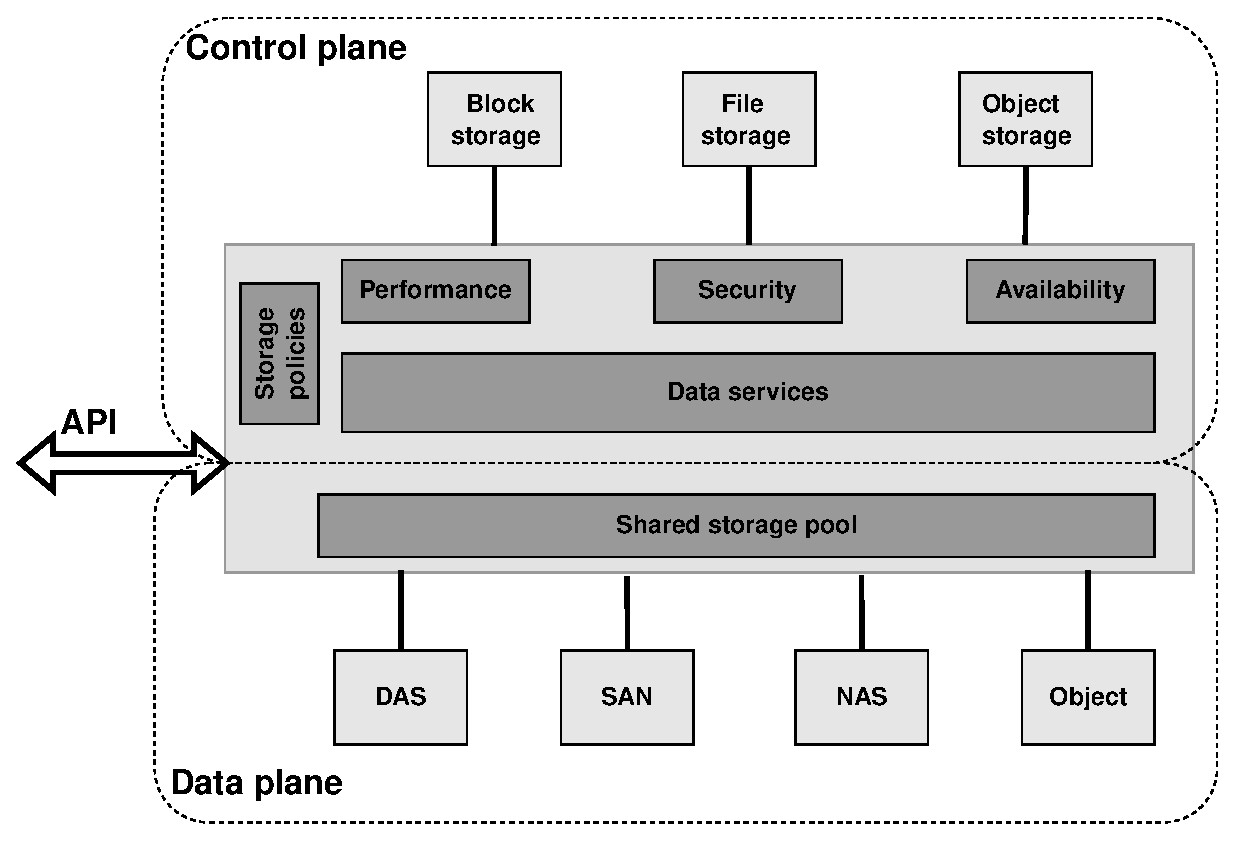
\includegraphics[width=1\textwidth]{obrazky-figures/sds-planes.eps}
        \caption{SDS data and control plane (source: \cite{sdsPlanes}, remade).}
        \label{fig:sdsPlanes}
    \end{figure}

\section{Beanstalk queue}

    Beanstalk queue or shorter \textbf{beanstalkd} is a fast, simple and lightweight working queue\cite{beanstalkdOfficial}. The primary use case is to manage workflow between different parts of workers of application through working queues and messages. Beanstalkd was developed for the need of Facebook application in order to reduce average response time\cite{beanstalkdOfficial}. Provided by simple protocol design, heavily inspired by Memcached, implemented in programming language C, Beanstalkd offers lean architecture, which allows it to be installed and used very simply, making it perfect for many use cases\cite{beanstalkdInstall}.


    \subsection{Beanstalkd elements}
    Beanstalkd is a priority queue with server-client architecture. The server represents queues where jobs are saved based on priority. Beanstalkd architecture is composed of several components:
    \begin{itemize}
        \item \textbf{Jobs} - tasks stored by the client
        \item \textbf{Tubes} - used for storing tasks, each tube contains a ready queue and a delay queue.
        \item \textbf{Producer} - creates and sends jobs to beanstalkd using command \texttt{put}.
        \item \textbf{Consumer} - process "listening" on an assigned tube, reserves and consumes jobs from the tube.
    \end{itemize}

    \subsection{Job Lifecycle}
    Each job is uniquely assigned to one worker at a time. The client creates a job and inserts it into a beanstalkd tube using the \texttt{put} command. While being in the tube, the job can be in next states\cite{beanstalkdProtocol}:
    \begin{itemize}
        \item \texttt{\textbf{Ready}} - the task is free and can be executed immediately by the Consumer.
        \item \texttt{\textbf{Delayed}} - the task has assigned delay time that needs to expire before execution. After delay time expires, beanstalkd will automatically change its state to \texttt{Ready}.
        \item \texttt{\textbf{Reserved}} - the task is reserved and is being executed by the \textit{Consumer}. Beanstalkd is responsible for checking whether the task is completed in time (\textbf{TTR} - Time to run).
        \item \texttt{\textbf{Buried}} - reserved task, the task will not be removed nor executed until the client decides. This state is often used for further inspection in debugging process when failure or undefined behavior occurs during task execution.
        \item \texttt{\textbf{Deleted}} - the task is deleted from the tube, beanstalkd no longer maintains these jobs.
    \end{itemize}

    Figure \ref{fig:beanstalkdJobSM} describes the life cycle of a job in a beanstalkd tube. Job is created by \textit{Producer} using put command. Beanstalkd allows the \textit{Producer} to add delay time before the task is ready for execution, setting the job state to \texttt{Delayed}. After delay time expires, beanstalkd will automatically change job state to \texttt{Ready}. The Producer can specify job priority and jobs with the \texttt{Ready} state are stored in the priority queue. A job with the biggest priority is reserved and executed by a \textit{Consumer}. After successfully executing the task, the \textit{Consumer} will delete the job from beanstalkd. If some error occurs, the \textit{Consumer} can \textbf{bury} the task. The Consumer can decide that he is not interested in completing the reserved task. Using the \texttt{release} command (with optional delay) job state will be changed back to \texttt{Ready} (or \texttt{Delay} if delay exists). Jobs with the \texttt{Burried} state will not be touched by the beanstalkd server until the client \texttt{"kicks"} them to \texttt{READY} state.

    \begin{figure}[H]
        \centering
        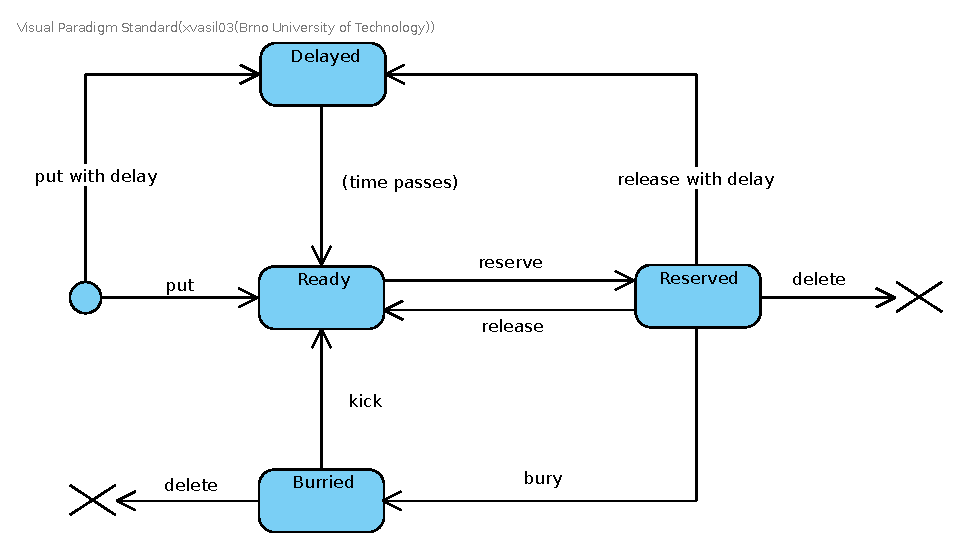
\includegraphics[width=1\textwidth]{obrazky-figures/beanstalkd-job-states.eps}
        \caption{State machine diagram of job in Beanstalkd tube.}
        \label{fig:beanstalkdJobSM}
    \end{figure}


    \subsection{Key characteristics}
    Key beanstalkd characteristics are:

    \paragraph{Asynchronous}- beanstalkd allows producers to put jobs in the queue, and workers can process them later.
    \paragraph{Distributed}- in the same way as \textit{Memcached}\footnote{Memcached - in-memory key-value store {\url{https://memcached.org/}}}, beanstalkd can be distributed, although this distribution is handled by clients. The beanstalkd server does not know anything about other beanstalkd running instances.
    \paragraph{Persistent}- beanstalkd offers support for persistent jobs during which all jobs are written to binlog. In case of a power outage, after restarting a beanstalkd instance, it will recover jobs content from the logs.
    \paragraph{Not secured}- beanstalkd is designed to be run in a private/secure network. Therefore it \textbf{does not support authentication or authorization}.
    \paragraph{Scalability}- beanstalkd can be scaled horizontally, although it must be done on the client side, where each client would connect to multiple servers and then use specific algorithms(e.g., Round-robin) to switch between the different servers.

\section{Event notifications}
    %introduction
     \textbf{An event} is a runtime operation executed by a software element, representing a significant change or occurrence in a system. Event is created in order to make some information available to other software elements not specified by the operation\cite{eventArchitecturalPatterns}.

    \textbf{Event notification} is a message created by a system in order to notify other parts of the system that an event has taken place\cite{eventRedHatEventDrivenArch}. Event notifications are usually used for monitoring and asynchronous job processing.

    In object storage, event notifications are used to notify users or tenants about specific changes and occurrences in their bucket or account. Typical event notifications include creating new (or updating existing) objects in the bucket. In addition, most object vendors offer \textbf{publish/subscribe} notifications, allowing users to subscribe to certain types of event notifications using predefined rules. Information about rules specifying event notifications is usually stored in the upper-level metadata (bucket or account).

    \subsection{CloudEvents}
    Publishers tend to describe event data differently due to non-existing standards or formats. The lack of a common way to describe events means developers have to learn how to handle events from each event source. To solve this problem, CloudEvents was created.

    \textbf{CloudEvents} is a specification for describing event data in common way\cite{eventCloudEvents} hosted by CNCF\footnote{CNCF - Cloud Native Computing Foundation {\url{https://www.cncf.io/}}}. CloudEvents goal is to dramatically simplify event specification and delivery across services, platforms and beyond.
    CloudEvents has been integrated by many popular object storage vendors, such as Oracle Cloud, IBM Cloud Code Engine, Azure, Google Cloud, etc.

    Attributes in CloudEvents specification can be divided into three categories:
    \paragraph{Required attributes} - set of attibures that are required to be included in all events\cite{eventCloudEventsSpec}:
    \begin{itemize}
        \item id (string) - event identifier, must not be empty.
        \item source (URI-reference) - identifies context in which event occured, must not be empty.
        \item specversion (string) - the version of CloudEvents specification, must not be empty.
        \item type (string) - value describing the type of occurred event. Often this attribute is used for policy enforcement, routing and monitoring.
    \end{itemize}

    \paragraph{Event data attirbutes} - attibures containing and describing event data:
    \begin{itemize}
        \item datacontenttype (string) - content type of data value (allows data to carry any type of content).
        \item dataschema (URI) - identifies the schema that data adheres to.
        \item data - data payload
    \end{itemize}

    \paragraph{Optional attributes}:
    \begin{itemize}
        \item time - timestamp
        \item subject (string) - the subject of the event in the context of the event producer.
        \item extension attributes - custom attibutes allowing external systems to attach metadata to an event.
    \end{itemize}

    \begin{lstlisting}[style=jsonStyle, caption=Example of event described using CloudEvents specification in JSON format.]
    {
        "specversion" : "1.0",
        "type" : "com.github.pull_request.opened",
        "source" : "https://github.com/cloudevents/spec/pull",
        "subject" : "123",
        "id" : "A234-1234-1234",
        "time" : "2018-04-05T17:31:00Z",
        "comexampleextension1" : "value",
        "comexampleothervalue" : 5,
        "datacontenttype" : "text/xml",
        "data" : "<much wow=\"xml\"/>"
    }
    \end{lstlisting}

    \subsection{Amazon S3 event notifications}
    \textbf{Amazon Simple Storage Service (S3)} is one of the most popular cloud object storages providing a \texttt{REST} web service interface. Amazon S3 is reliable, scalable, commercial and one of the most popular object storage that manages Web-Scale computing by itself\cite{eventS3}. As a result, Amazon S3 has a big impact on object storage and most other object storage vendors crated compatible \textbf{S3 API} for their services.

    One of the monitoring features that Amazon S3 provides is \textbf{Event Notification}, which offers users to receive notifications when certain events happen in their S3 bucket. To enable such notifications, users need to create a notification configuration that identifies which events Amazon S3 should publish\cite{eventS3EventNotification}. Notifications are configured at the bucket level and then applied to each object in the bucket.

    Amazon S3 provides limited event destinations to which event notification messages can be send\cite{eventS3EventNotificationDest}:
    \begin{itemize}
        \item \textit{Amazon Simple Notification Service (Amazon SNS)} - flexible, fully managed push messaging service, can be used to send messages to mobile phones or distributed services.
        \item \textit{Amazon Simple Queue Service (Amazon SQS)} queues - reliable and scalable hosted queues for storing messages as they travel between computers.
        \item \textit{AWS Lambda} - serverless, event-driven compute service. Lambda can run custom code in response to the Amazon S3 bucket event (if the lambda function writes to the same bucket that triggers the notification, it can create an execution loop).
        \item \textit{Amazon EventBridge} - serverless event bus service used to receive events from AWS. It allows users to define rules to match events and deliver them to defined targets.
    \end{itemize}

    By this date, Amazon S3 \textbf{does not support CloudEvents} specification and describes event data in its own way. Some of the event types that Amazon S3 can publish are displayed in table \ref{tab:eventTypesS3}.


     \renewcommand*{\arraystretch}{1.4}
     \begin{table}[H]
     \begin{tabularx}{\textwidth}{|p{0.3\textwidth}|X|}
         \hline
         \textbf{Event type} & \textbf{Desription} \\
         \hline
         s3:TestEvent & after enabling the event notifications, Amazon S3 publishes a test notification to ensure that topic exist and bucket owner has permissions to publish specified topic. \\
         \hline
         s3:ObjectCreated:* & An object was created (regardless on operation). \\
         \hline
         s3:ObjectCreated:Put & An object was created by an HTTP PUT operation. \\
         \hline
         s3:ObjectCreated:Post & An object was created by HTTP POST operation. \\
         \hline
         s3:ObjectCreated:Copy & An object was created an S3 copy operation. \\
         \hline
         s3:ObjectCreated:

         CompleteMultipartUpload & An object was created by the completion of a S3 multi-part upload. \\
         \hline
         s3:ObjectRemoved:* & An object was removed (regardless on operation). \\
         \hline
         s3:ObjectRemoved:Delete & An object was deleted by HTTP DELETE operation. \\
         \hline
         s3:ObjectRemoved:

         DeleteMarkerCreated & An versioned object was marked for deletion. \\
         \hline
    \end{tabularx}
    \caption{Subset of Amazon S3 Event Types \cite{eventS3EventNotificationDest}\label{tab:eventTypesS3}}
    \end{table}


\chapter{OpenIO SDS}\label{chap:openiosds}
    This chapter introduces OpenIO Software-defined storage, its key features, its data organization along with the underlying technologies. Furthermore, this chapter introduces Grid For Apps framework (\ref{sec:oioGridForApps}) and event publishing in OpenIO (\ref{sec:oioEvent-Agent}).

    OpenIO Software-defined storage is open source object storage that is perfectly capable of traditional use cases (such as archiving, big data, cloud). However, at the same time, combined with Grid for Apps (\ref{sec:oioGridForApps}), it opens the door for users to create an application that needs much more sophisticated back-end operations. These applications include industrial IoT, machine learning and artificial intelligence, as well as any other applications whose workflow can benefit from automated jobs or tasks\cite{oioNextGen}. In addition, OpenIO SDS is event-driven storage with the ability to intercept events seamlessly and transparently to the rest of the stack.

    \section{Key characteristics}
    \subsection*{Hardware agnostic}
    OpenIO SDS is fully software-defined storage capable of running on x86 or ARM hardware with minimal requirements. Cluster nodes can be different from each other, allowing different generations, types, and capacities to be combined without affecting a performance or efficiency\cite{oioKeyChars}.
    OpenIO has built-in support for heterogeneous hardware allowing every node to be used at its maximum performance.
    \subsection*{No SPOF architecture}
    Every single service used to serve data is redundant from object chunks stored in a disc to the directory level, every information is duplicated. As a result, there is no single point of failure (SPOF) in the cluster and a node can be shut down without affecting overall availability or integrity\cite{oioCoreSolution}.
    \subsection*{Cluster organization}
    Instead of a traditional cluster ring-like layout, OpenIO SDS is based on a grid of nodes \ref{fig:oioArch}. It is flexible and resource-conscious. Compared to other object storage solutions, cluster organization is not based on static data allocation that usually use Chord peer-to-peer distributed hash table algorithm. Instead, OpenIO SDS uses distributed directory for organizing data and metadata hash tables, which allows the software to attain the same level of scalability but with better and more consistent performance\cite{oioKeyChars}.

    \begin{figure}[H]
        \centering
        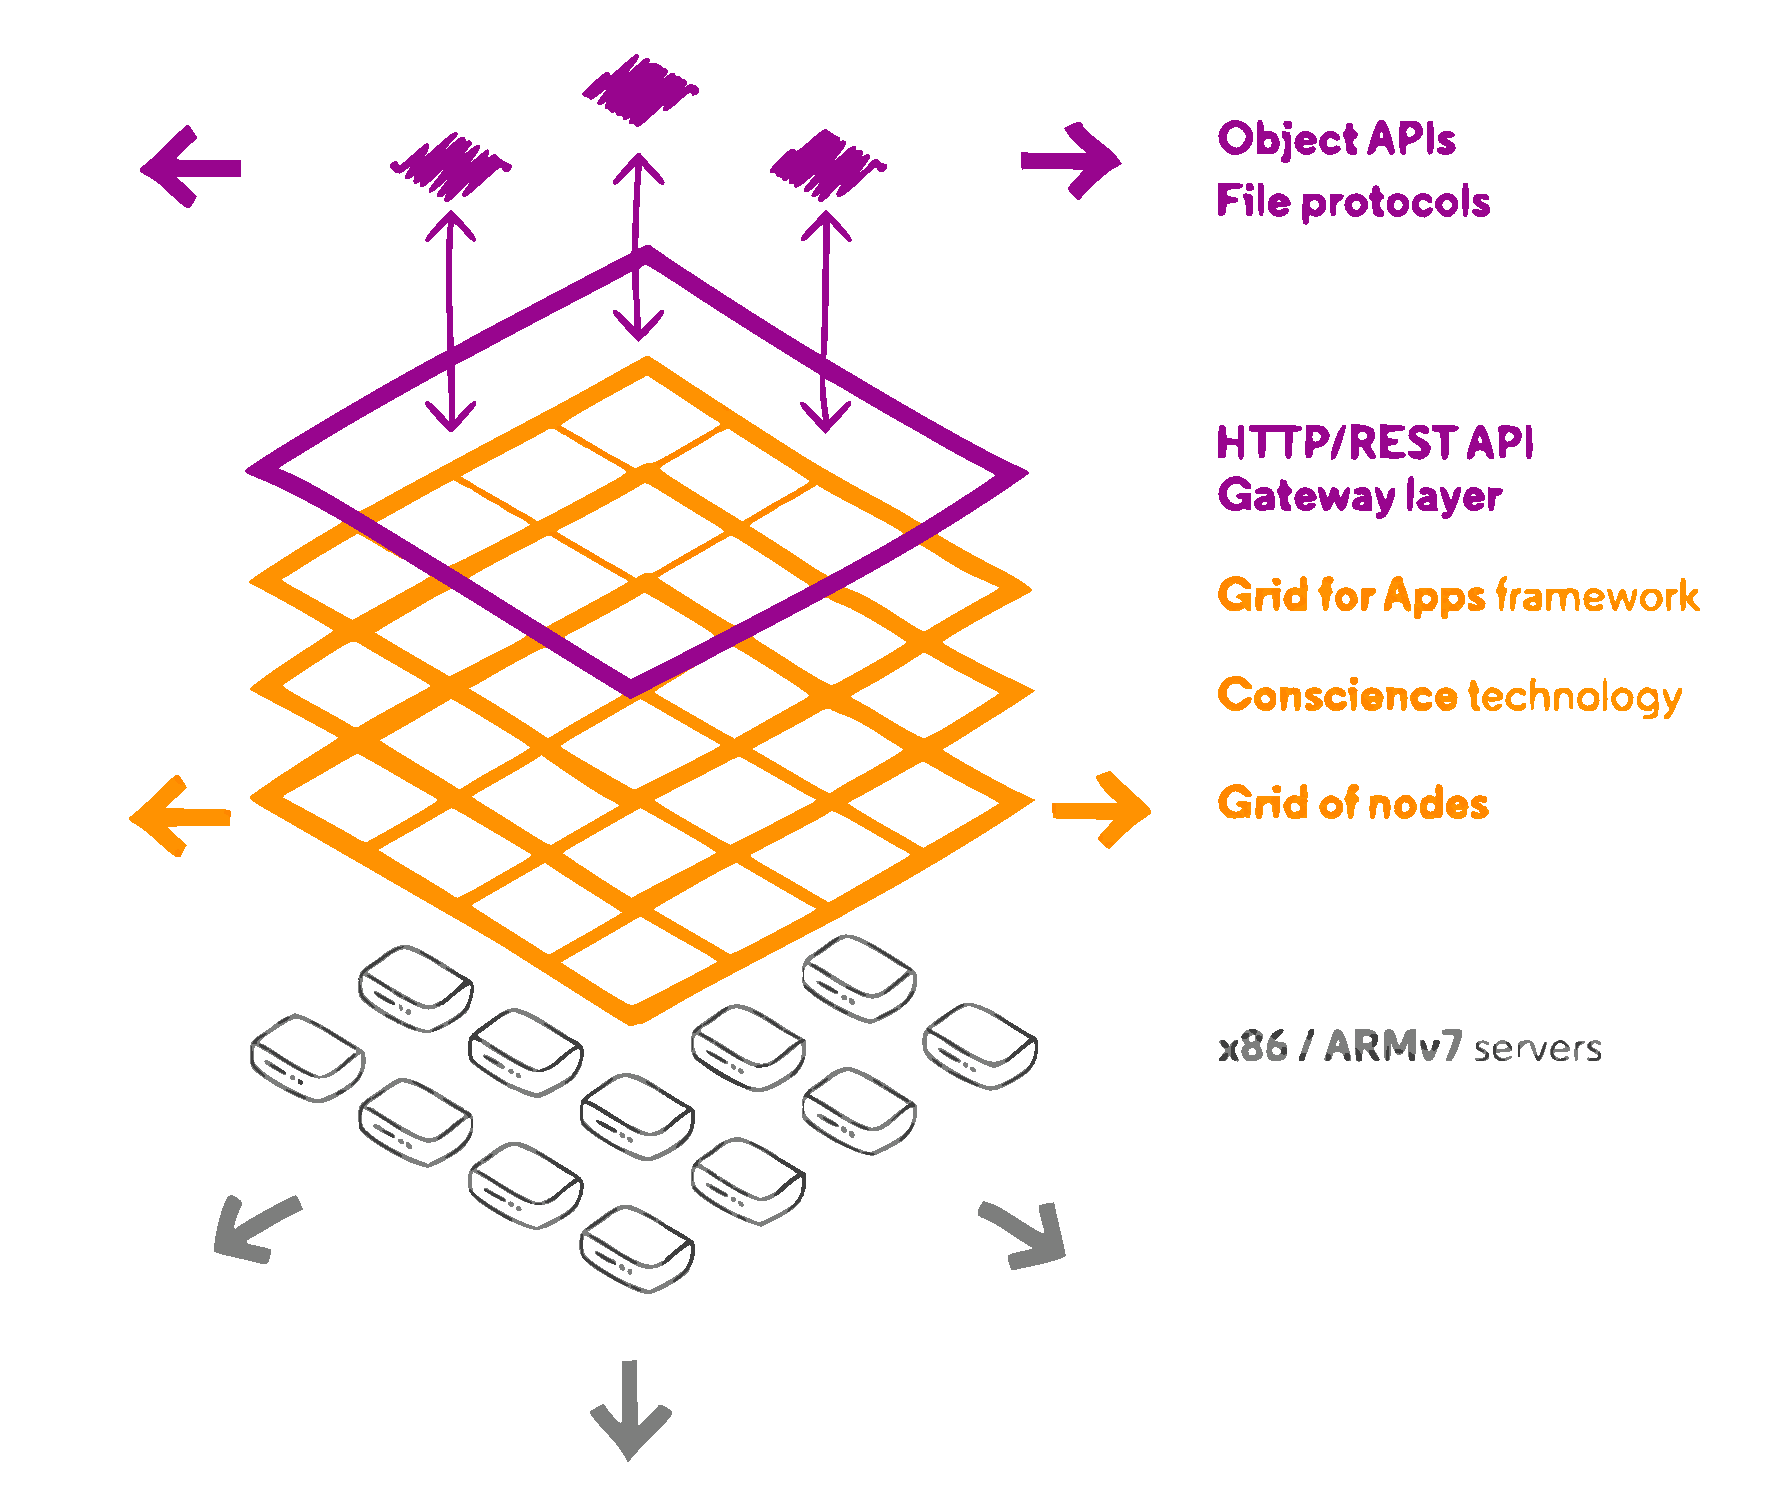
\includegraphics[width=1\textwidth]{obrazky-figures/openio-architecture.eps}
        \caption{Layered view on OpenIO SDS architecture (source: \cite{oioArch}).}
        \label{fig:oioArch}
    \end{figure}


    \subsection*{Tiering}
    With tiering, OpenIO SDS offers users to configure a pool containing a group of hardware that can then be used to store specific types of objects. For example, users can create a pool of high-performance hard disks (e.g. SSDs) and use the pool to store objects that require low latency.
    This feature is realized by a mechanism called \textbf{storage policies}. Multiple storage policies can be defined in one particular namespace. Storage policies can also be used for specifying how many replicas should be created for a specific dataset\cite{oioCoreSolution}.

    \subsection*{ConsciousGrid}
    ConsciousGrid is an OpenIO technology that uses real-time metrics from the nodes(CPU, I/O, capacity) automatically discover and place data in the most appropriate place. It provides \textbf{load balancing} and computes a score for each node and then provides weighted random selection\cite{oioSdsServices}.


    \section{Data organization}
    Multi-tenancy is one of the core concepts in OpenIO SDS. Data objects are stored within following hierarchy: \texttt{Namespace/Account/Container/Object} \ref{fig:oioDataOrganization}. Multiple namespaces can be configured in each cluster, providing multi-region/zone logical layouts for applications and segregated workloads depending on a tenant or geo-distribution need\cite{oioSdsConcepts}.
    There is no classic subdirectory tree. Instead, objects are stored in a flat structure in the container level. However, like many other object storages, there is a way to emulate a filesystem.

    \begin{figure}[H]
        \centering
        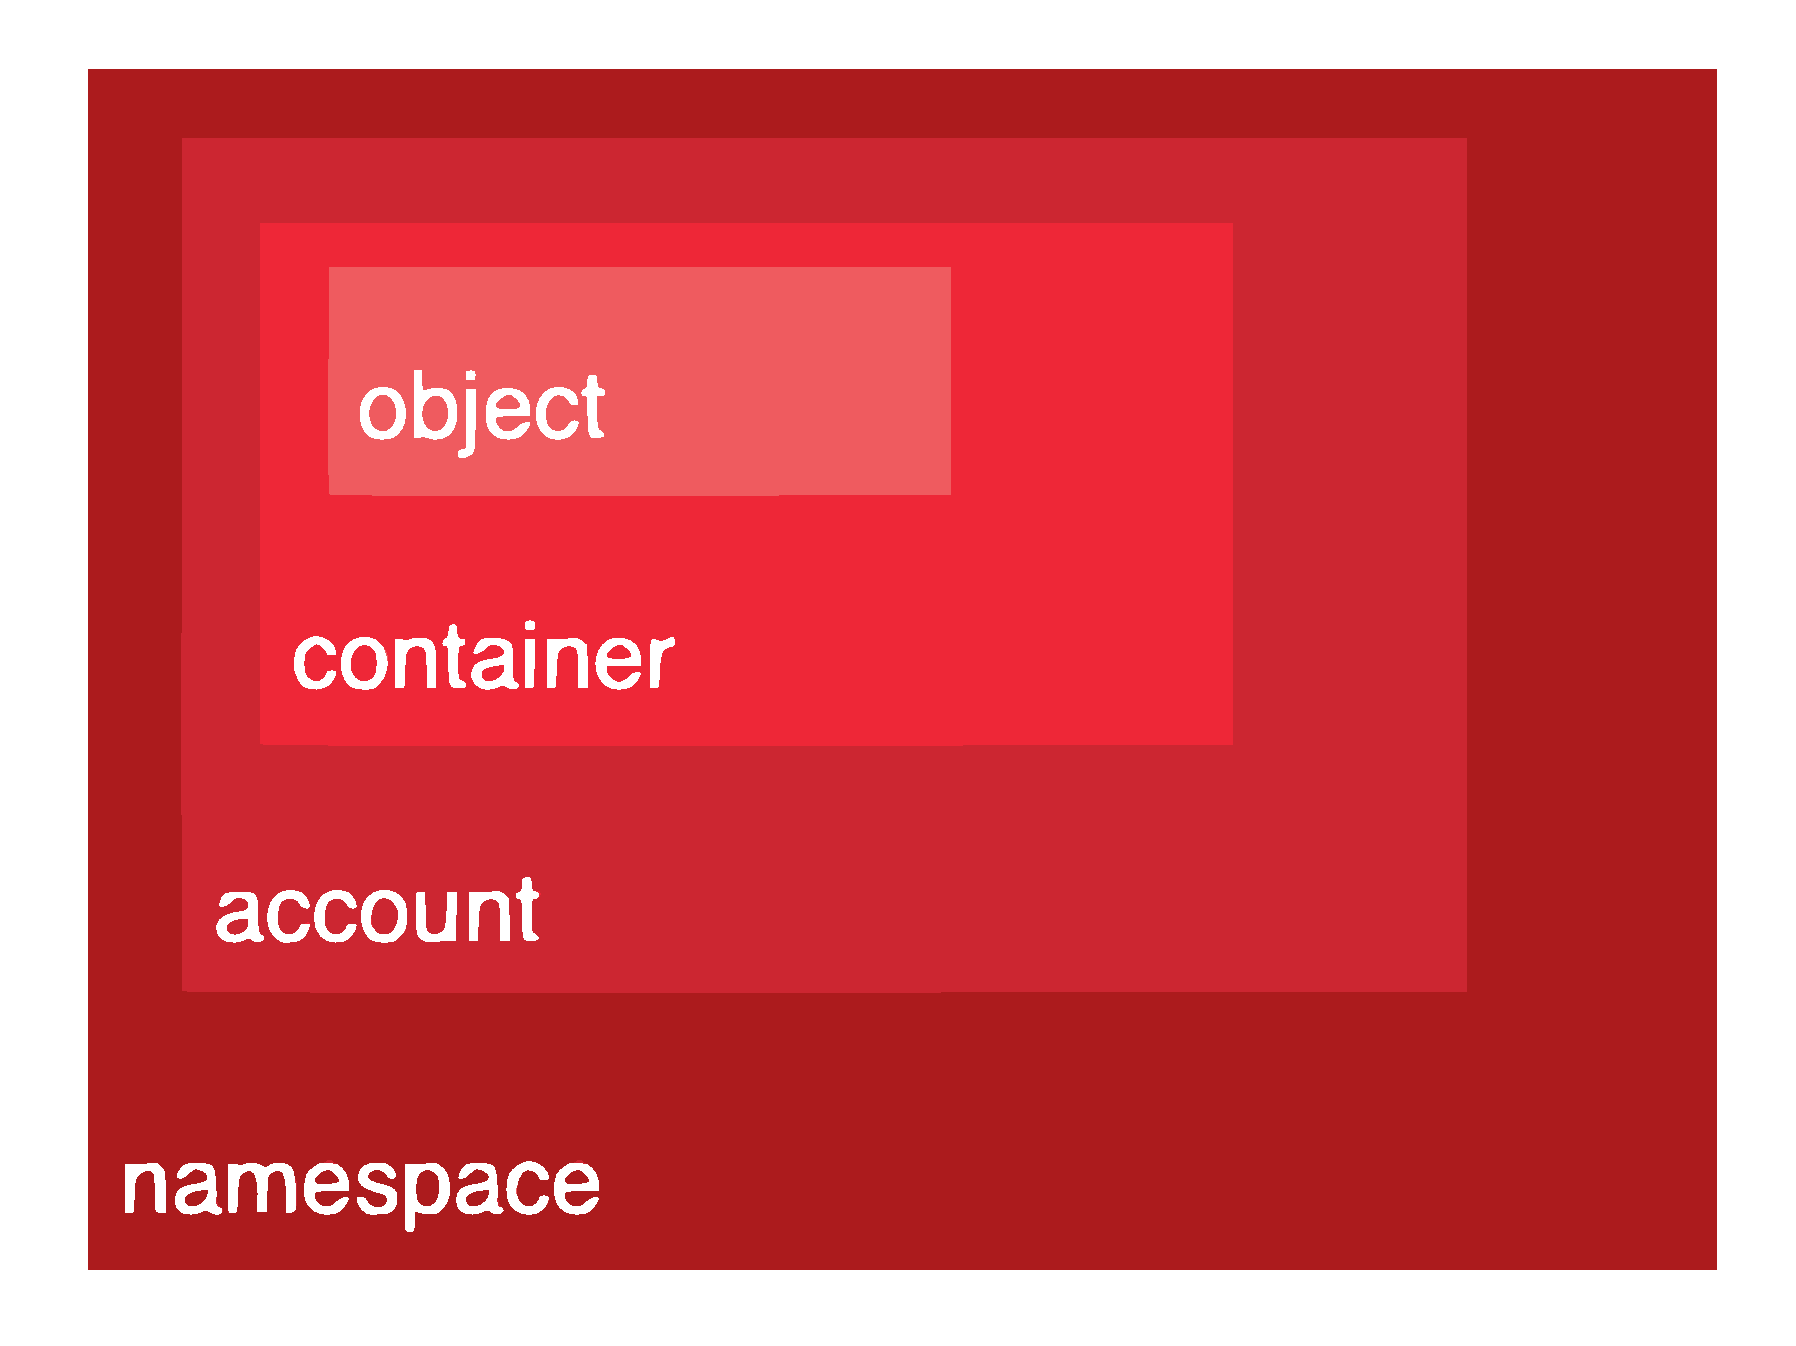
\includegraphics[width=0.5\textwidth]{obrazky-figures/openio-data-organization.eps}
        \caption{Object data organization in OpenIO SDS (source: \cite{oioCoreSolution}).}
        \label{fig:oioDataOrganization}
    \end{figure}

    \subsection{Namespace}
    A coherent set of network services working together to run OpenIO's solutions. It hosts services and provides operations such as service configuration and monitoring.

    \subsection{Account}
    An account usually represents a tenant and is the top level of data organization. Each account owns and manages a collection of containers. In addition, the account keeps track of namespace usage for each customer (i.e. bytes occupied by all of a customer's objects)\cite{oioCoreSolution}.

    \subsection{Container}
    Container represents an object bucket. Each container belongs to one (and only one) account and is identified by a unique name within the account. The container carries additional information specifying how to manage its objects (e.g. how to secure them)\cite{oioCoreSolution}.

    \subsection{Object}
    Object is the smallest data unit visible by a customer and represents a named BLOB with metadata. OpenIO SDS allows several objects to be stored in a container and are considered versions of the same object. Classic \texttt{API} operations (\texttt{PUT/GET/DELETE}) will be directed towards an object with the latest version. If the size of an object is larger than the specified limit at the namespace level, the object will be divided into chunks of data. This behavior allows capacity optimization as well as \textbf{distributed reads} that could be particularly useful for high-speed video streaming of large media\cite{oioCoreSolution}.

    %todo authentication and acl?

    %\section{Services} maybe include?
    \section{Serverless computing}
    OpenIO offers Serverless computing in object storage cluster nodes using the framework Grid For Apps.
    \subsection{Grid For Apps}\label{sec:oioGridForApps}

    Like Amazon AWS Lambda, OpenIO offers an \textbf{event-driven compute service} called Grid for Apps that works on top of OpenIO.

    Grid for Apps intercepts all the events that happen in the storage layer, and based on user configuration, triggers specific applications or scripts to act on data (metadata) stored in object storage\cite{oioNextGen}. The application is executed in cluster nodes and utilizes free unused resources available in the cluster. This improves efficiency (fewer data moving since object data are already available) and saves money (no need for external resources)\cite{oioNextGen}.

    Grid for Apps allows customers to perform operations such as metadata enrichment, data indexing and search (e.g. indexing metadata to Elasticsearch), pattern recognition, machine learning, data filtering, monitoring, etc\cite{oioNextGen}.

    Grid for Apps in OpenIO is realized using service \texttt{event-agent} and \texttt{beanstalkd} queue.

    \subsection{Event-agent}\label{sec:oioEvent-Agent}
    Event-agent is an OpenIO service responsible for handling asynchronous jobs. It relies on beanstalkd backend to manage jobs. Event-agent key characteristics are\cite{oioSdsServices}:
    \begin{itemize}
        \item Stateless
        \item CPU intensive
        \item Must be deployed on every server of the cluster
    \end{itemize}

    Every event that occurs in OpenIO is inserted in a beanstalkd tube. Event-agent is listening to the beanstalkd tube and consumes jobs from it. Consumers are produced using Eventlet Network Library \cite{oioEventlet}. The number of workers can be configured.

    In event-agent, users can specify handlers for each type of event in event-handler.conf.
    Some of the event types in OpenIO are \texttt{storage.content.new} (e.g., new object in storage), \texttt{storage.container.deleted} (e.g., object has been deleted), etc.

    \textbf{Events handler} is defined as a pipeline containing applications that will react to the event. In example \ref{lst:event-agent-handlers}, deleting an object will invoke \texttt{storage.content.deleted} event. Event-agent will handle the event using \texttt{content\_cleaner} application, which deletes objects chunks from object storage.

    OpenIO offers users to process events outside of the event-agent. In order to do that, users can use the application \texttt{notify} which will send an event to a specified beanstalkd tube. Then a user can create a custom consumer process that will execute the job from beanstalkd tube. An example of such configuration is displayed in listing \ref{lst:event-agent-handlers}.

    \lstset{
        caption=Example of event-agent handler configuration,
        label=lst:event-agent-handlers
    }
    \begin{minipage}{\linewidth}
    \begin{lstlisting}
    [handler:storage.content.deleted]
    pipeline = content_cleaner

    [handler:storage.content.new]
    pipeline = notify

    [filter:content_cleaner]
    use = egg:oio#content_cleaner

    [filter:notify]
    use = egg:oio#notify
    tube = oio-rebuild
    queue_url = ${QUEUE_URL}
    \end{lstlisting}
    \end{minipage}

\chapter{OpenStack Swift}\label{chap:swift}
    This chapter introduces OpenStack object storage (code name Swift) and describes its key features. Furthermore, this chapter elaborates OpenStack Swift architecture, introduces its main services and interfaces for communication with object storage.

    OpenStack Swift is open-source object storage developed by Rackspace, a company that, together with NASA, created the OpenStack project. After becoming an open-source project, Swift became the leading open-source object storage supported and developed by many famous IT companies, such as Red Hat, HP, Intel, IBM, and others.

    OpenStack Swift is a multi-tenant, scalable, and durable object storage capable of storing large amounts of unstructured data at low cost\cite{swiftOpenStackSwift}.

    \section{Key characteristics}
    Besides standard object storage characteristics (like scalability, durability, hardware agnostic, etc.), some of the keys OpenStack Swift characteristics:

    \paragraph{Multi-regional capability}
    OpenStack Swift has distributed architecture. Data can be distributed and replicated into multiple data centers, although the negative effect could be higher latency between them. Distribution can provide high availability of data and recovery site\cite{swiftOpenStackSwift}.

    \paragraph{No SPOF}
    With all data being replicated and distributed, there is no single proof of failure in OpenStack Swift architecture.

    \paragraph{Developer-friendliness}
    OpenStack Swift offers many built-in features that developers and users can use. some of the most interesting built-in features are\cite{swiftOpenStackSwift}:
    \begin{itemize}
        \item \textbf{Automatically expiring objects} - Objects can be given expiration time, after which objects become invalid and deleted from object storage.
        \item \textbf{Quotas} - Storage limits can be configurated on container/account level.
        \item \textbf{Versioned objects} - User can store a new version of an object, while object storage keeps previous (older) versions.
        \item \textbf{Access control lists} - Users can configure access to their data to give or deny permission for reading or writing data to other users.
    \end{itemize}

    \paragraph{Middleware support}
    - OpenStack Swift allows adding custom middlewares, which will be run directly on storage system\cite{swiftEssentials}. This feature can be used for monitoring purposes, for example, informing users or other applications about new objects in storage using Webhook middleware.

    \paragraph{Large object support}
    - By default, OpenStack Swift has a limit on a single uploaded object, which is 5GB. However, using segmentation, the size of a single object can be virtually unlimited. This option offers a possible higher upload speed, in case of parallel upload\cite{swiftLOS}.

    \paragraph{Partial object retrival}
    Users can retrieve part of an object, for example, just a portion of a movie object file\cite{swiftImplementingCloudStorage}.

    \section{Data model}
    OpenStack Swift allows users to store unstructured data objects with a canonical name containing \textit{account}, \textit{container} and \textit{object} in given order\cite{swiftOpenStackSwift}. The account names must be unique in the cluster, the container name must be unique in the account space, and the object names must be unique in the container. Other than that, if containers have the same name but belong to a different account, then they represent different storage locations. The same principle applies to objects. If objects have the same name but not the same container and account name, then these objects are different.

    \subsection{Account}
    Accounts are root storage locations for data. Each account contains a list of containers within the account and metadata stored as key-value pairs. Accounts are stored in the account database. In OpenStack Swift, account is \textbf{storage account} (more like storage location) and \textbf{do not represent a user identity}\cite{swiftOpenStackSwift}.

    \subsection{Container}
    Containers are user-defined storage locations in the account namespace where objects are stored. Containers are one level below accounts, therefore they are not unique in the cluster. Each container has a list of objects within the container and metadata stored as key-value pairs. Containers are stored in container database\cite{swiftOpenStackSwift}.

    \subsection{Object}
    An object represents data stored in OpenStack Swift. Each object belongs to one (and only one) container. An object can have metadata stored as key-value pairs. Swift stores multiple copies of an object across the cluster to ensure durability and availability. Swift does this by assigning an object to \textit{partition}, which is mapped to multiple drives, and each driver will contain object copy\cite{swiftOpenStackSwift}.

    \section{Server Processes}
    The path towards data in OpenStack Swift consists of four main software services: \textbf{Proxy server}, \textbf{Account server}, \textbf{Continaer server} and \textbf{Object server}. Typically Account, Container and Object server are located on same machine creating \textbf{Storage node}.

    \subsection{Proxy server}
    The proxy server is the service responsible for communication with external clients. For each request, it will look up storage location(node) for an account, container, or object and route the request accordingly\cite{SwiftArchitecturalOverview}. The proxy server is responsible for handling many failures. For example, when a client sends a \texttt{PUT} request to OpenStack Swift, the proxy server will determine which nodes store the object. If some node fails, a proxy server will choose a hand-off node to write data. When a majority of nodes respond successfully, then the server proxy will return a success response code\cite{swiftOpenStackSwift}.

    \subsection{Account server}
    Account server stores information about containers in a particular account to SQL database. It is responsible for listing containers. It does not know where specific containers are, just what containers are in an account\cite{SwiftArchitecturalOverview}.

    \subsection{Container server}
    Container server is similar to account server, except it is responsible for listing objects and also does not know where specific objects are\cite{SwiftArchitecturalOverview}.

    \subsection{Object server}
    The Object Server is blob storage capable of storing, retrieving, and deleting objects. Objects are stored as binary files to a filesystem, where metadata are stored in the \textit{file's extended attributes (xattrs)}. This requires a filesystem with support of such attributes. Each object is stored using a hash value of object path (account/container/object) and timestamp. This allows storing multiple versions of an object. Since last write wins (due to timestamp), it is ensured that the correct object version is served\cite{SwiftArchitecturalOverview}.

    \begin{figure}[H]
        \centering
        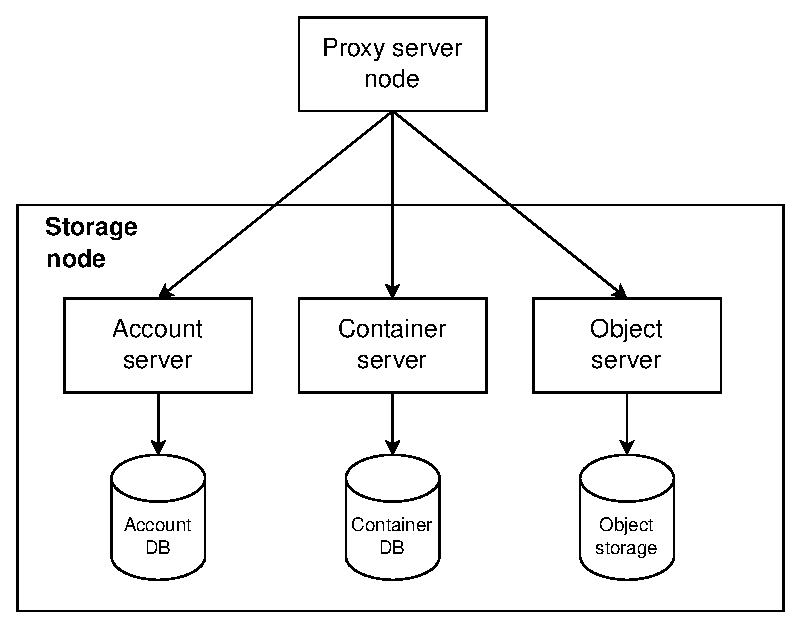
\includegraphics[width=0.75\textwidth]{obrazky-figures/swift-servers.eps}
        \caption{OpenStack Swift servers architecture.}
        \label{fig:swiftServers}
    \end{figure}

    \section{Middlewares}
    Using Python WSGI middleware, users can add functionalities and behaviors to OpenStack Swift. Most middlewares are added to the Proxy server but can also be part of other servers (account server, container server, or object server).

    Middlewares are added by changing the configuration of servers. In example \ref{lst:swiftMiddleware}
    \texttt{webhook middleware} is added into the proxy server by changing its pipeline (\textit{pipeline:main}). Middlewares are executed in the given order (first will be called webhook middleware, then proxy-server middleware).

    Some of the middlewares are required and will be automatically inserted by swift code\cite{swiftMiddleware}.

    \lstset{
        caption=Example of proxy server configuration (proxy-server.conf).,
        label=lst:swiftMiddleware
    }
    \begin{lstlisting}
    [DEFAULT]
    log_level = DEBUG
    user = <your-user-name>

    [pipeline:main]
    pipeline = webhook proxy-server

    [filter:webhook]
    use = egg:swift#webhook

    [app:proxy-server]
    use = egg:swift#proxy
    \end{lstlisting}

    \subsection{Interface}
    OpenStack Swift servers are implemented using Python WSGI applications. Therefore only Python WSGI middlewares are accepted in OpenStack Swift.

    In \ref{lst:swift-healthcheck} is example of simplified \texttt{healthcheck middleware}. The constructor takes two arguments, the first is a WSGI application, and the second is a configuration of middleware defined using Python Paste framework in \texttt{proxy-server.conf}. Middleware must have a call method containing the request environment information and response from previously called middleware. Middleware can perform some operations and call the next middleware in the pipeline or intercept a request. In the healtcheck example, if the path directs to \texttt{/healtcheck} , the middleware will return \texttt{HTTP Response}, and other middlewares in the pipeline will not be called.

    Method \texttt{filter\_factory} is used by the Python Paste framework to instantiate middleware.

\begin{lstlisting}[language=Python, style=pythonStyle, caption=Example of healthcheck middleware in OpenStack Swift, label=lst:swift-healthcheck]
import os
from swift.common.swob import Request, Response

class HealthCheckMiddleware(object):
    def __init__(self, app, conf):
        self.app = app

    def __call__(self, env, start_response):
        req = Request(env)
        if req.path == '/healthcheck':
            return Response(request=req, body=b"OK", content_type="text/plain")(env, start_response)
        return self.app(env, start_response)

def filter_factory(global_conf, **local_conf):
    conf = global_conf.copy()
    conf.update(local_conf)

    def healthcheck_filter(app):
        return HealthCheckMiddleware(app, conf)
    return healthcheck_filter
\end{lstlisting}

    \subsection{Metadata}
    OpenStack Swift separates metadata into 3 categories based on their use:
    \begin{itemize}
        \item \textbf{\texttt{User Metadata}} - User metadata takes form \texttt{X-<type>-Meta-<key>: <value>}, where \texttt{<type>} represent resource type(i.e. account, container, object), and \texttt{<key>} and \texttt{<value>} are set by user. User metadata remain persistent until are updated using new value or removed using header \texttt{X-<type>-Meta-<key>} with no value or a header \texttt{X-Remove-<type>-Meta-<key>: <ignored-value>}.
        \item \textbf{\texttt{System Metadata}} - System metadata takes the form of \texttt{X-<type>-Sysmeta-<key>: <value>}, where \texttt{<type>} represent resource type(i.e. account, container, object) and \texttt{<key>} and \texttt{<value>} are set by internal service in Swift WSGI Server.
        All headers containing system metadata are deleted from a client request.

        System metadata are visible only inside Swift, providing a means to store potentially sensitive information regarding Swift resources.
        \item \textbf{\texttt{Object Transient-Sysmeta}} - System metadata takes the form of \texttt{\newline X-Object-Transient-Sysmeta-<key>:<value>}. Transient-sysmeta has a similar behavior as system metadata and can be accessed only within Swift, and headers containing Transient-sysmeta are dropped. If middleware wants to store object metadata, it should use transient-sysmeta\cite{swiftMiddleware}.
    \end{itemize}

\chapter{MinIO}\label{chap:minio}
This chapter introduces MinIO object storage, describes its key features, most essential components, and event notifications in MinIO.

\section{Introduction}
    MinIO is software-defined object storage that provides high performance and scalability. MinIO was designed to be the standard in private/hybrid cloud object storage.
    It runs on industry-standard hardware and is 100\% open source\cite{minioObjectStorage}.

    MinIO software-defined object storage suite consists of a \textit{MinIO server} and optional components.

    \paragraph{MinIO Server} - MinIO Server is distributed object storage server.
    \paragraph{MinIO Client} - Service provoding familiar UNIX commands like \textit{ls, cat, cp, diff} in MinIO storage.
    \paragraph{MinIO Console} - Browser-based GUI offering all commands from MinIO Client in a design that feels more intuitive for DevOps and IT admins.
    \paragraph{MinIO Kubernetes Operator} - plugin allowing easy deployment and operation of MinIO object storage on Kubernetes.

\section{Key features}
    MinIO was designed to multiple benefits to object storage:

    \subsection*{Ease of use}
    MinIO can be installed simply by downloading a single binary file and executing it. The configuration setup has been kept to a bare minimum. Upgrading to a newer version is done with a single command, which is non-disruptive and does not provoke any downtime\cite{minioIntel}.

    \subsection*{Encryption and WORM}
    MinIO provides per-object encryption using a unique object key protected by a master key managed key-management system (KMS).

    MinIO supports object locking by enforcing \textit{Write-Once-Read-Many(WORM)} immutability until the lock is expired or lifted. This mode prevents tempering with data once written\cite{minioHighPerformance}.

    \subsection*{Metadata architecture}
    MinIO does not provide separate storage for metadata. All operations are performed on object-level granularity. This approach isolates any failures and does not allow any spillover to larger system failures\cite{minioIntel}.

    \subsection*{High availability}
    MinIO design allows a server to lose up to half its drivers and a cluster to lose up to half its servers, and MinIO will still be able to successfully process requests and serve objects. This is achieved by erasure code that protects data with redundancy\cite{minioIntel}.

\section{Event notifications}
    MinIO supports event notification for an event occurring to objects. MinIO provides Amazon S3 like events structure and API for defining which events will be published. Users can use the MinIO client or provided MinIO SDK API to set event configuration.

    Supported event notification targets are AMQP, Redis, MySQL, LMQTT, NATS, Apache Kafka, Elasticsearch, PostgreSQL, Webhooks, and NSQ.

    Beside events occred on objects such as \texttt{s3:ObjectCreated:*} and \texttt{s3:ObjectRemoved:*}, MinIO offers event notification for access to storage \texttt{s3:ObjectAccessed:*} and event notification when bucket is created \texttt{s3:BucketCreated} and deleted \texttt{s3:BucketRemoved}.


\chapter{Solution draft}\label{chap:solution}
    This chapter describes the current state of event notifications in OpenIO SDS, OpenStack Swift, and MinIO. It describes proposed solutions for OpenIO SDS and OpenStack Swift in the form of middleware and for publishing events notification from MinIO to Beanstalkd in the form of an proxy application.
\section{Current state}
    \subsection{OpenIO SDS}
    OpenIO Software-Defined storage has event-driven architecture, capable of publishing events to Beanstalkd using \textit{event-agent service} and \textit{Notify filter}.
    The main disadvantage of the current event publishing state is that configuration describing what type of events should be published is applied to the whole storage. Since OpenIO SDS is a multi-tenant space, some tenants might be interested in different events inside storage. The best use-case solution would be to let tenants decide what kind of events should be published in storage assigned to them.

    Second disadvantage is \textbf{lack of event filters}. Tenants might be interested in events involving specific objects or buckets that satisfy specific rules (e.g., object prefix, size).

    The third disadvantage is that events are published only to a beanstalkd queue. OpenIO SDS does not support any other destinations for event publishing. Since events can be used for monitoring, there should be a proper interface, allowing users to define the destination to which events will be published (e.g., Kafka, Prometheus, MySQL).

    \subsection{OpenStack Swift}
    Currently, there is support for event publishing in OpenStack Swift. For example, there is no way to detect changes in a given container except by listing its content and comparing timestamps.

    To partially solve this problem, OpenStack Swift created a specification of middleware that would send out notifications to users if a new object was created, metadata updated, or data has been deleted.
    Two proposed solutions lacked a standard interface for event publishing (no support for either Amazon S3 or CloudEvents), which were not accepted and are outdated.

    \subsection{MinIO}
    MinIO supports event publishing in the form of \textit{Bucket notifications}. It can inform a user when an object is created, updated, or deleted. Besides events regarding objects, MinIO provides events notifications for replication events and evens regarding creating and deleting buckets. Furthermore, MinIO allows users to configure which events will be published using the Amazon S3 event notification structure.

    MinIO offers various notification targets (e.g., MySql, Redis, Elasticsearch) but does not offer Beanstalkd as a notification target.

    Minio is open-source object storage but \textbf{does not provide custom middlewares}. However, since MinIO is implemented in the Go programming language, any custom changes (tweaks) in MinIO source code means that the whole project needs to be compiled, which can result in incompatibility in future versions of MinIO.

\section{Middleware for OpenStack Swift and OpenIO SDS}
    The goal is to create common application/middleware capable of running within OpenStack Swift and OpenIO SDS. The middleware will allow users to configure: which types of events will be published and a destination where given events will be published. Proposed middleware will be called \textbf{\texttt{EventNotification}}.

    \subsection{Location}
    For OpenIO SDS ideal place to run new middleware is inside the pipeline of event-agent. The main reason is that the event-agent has access to every event that occurs in OpenIO SDS and processes jobs in asynchronous mode, which means it will not impact the latency of client requests.

    Most of the middlewares within OpenStack Swift are placed in the Proxy server since they can react to every client request. Therefore, the new proposed middleware will also be placed inside the Proxy server pipeline.

    \subsection{Design}
    The proposed middleware heavily utilizes containers/buckets and accounts metadata. Information about which event should be published and where will be stored in metadata of upper level. For publishing events regarding objects, the configuration will be stored in a container/bucket metadata (for container/bucket events, the configuration will be stored in the account level).

    Compared to Amazon S3 Notifications, EventNotification middleware will publish events regarding containers/buckets. Furthermore, EventNotification middleware will publish events regarding access to object storage (HTTP GET/HEAD), where Amazon S3 only offers notifications about changes (PUST/POST) in a bucket.

    EventNotification middleware can be configured so that specific even types will be forbidden for publishing in whole object storage. This option could be beneficial when there are many reads from object storage, and publishing those events could significantly impact object storage performance. Therefore such event types can be disabled for whole object storage.

    Activity diagram of EventNotification middleware in container level is shown in figure \ref{fig:middlewareActivity}. Container metadata contains event notification configuration for publishing objects in a given container. Therefore the first step is to parse and validate such metadata. If the event notification configuration is not valid, then such configuration will be removed from metadata.
    \begin{figure}[H]
        \centering
        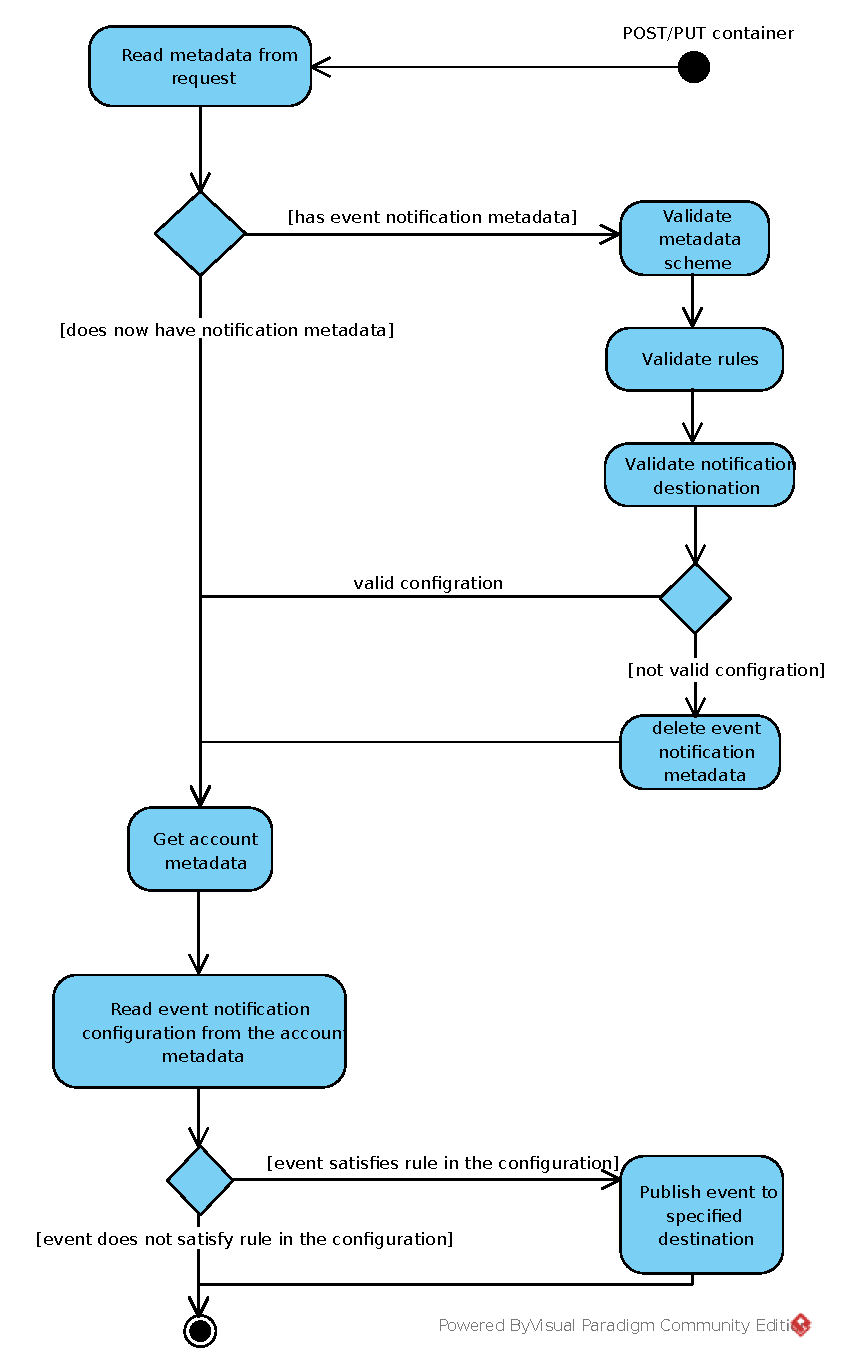
\includegraphics[width=0.8\textwidth]{obrazky-figures/middleware-activity-diagram.eps}
        \caption{Acitiviy diagram of EventNotification middleware.}
        \label{fig:middlewareActivity}
    \end{figure}
    The next step is deciding if the event should be published. Since metadata about event publishing is stored in the upper level, EventNotification needs to read account metadata from storage. After reading and parsing account metadata, \texttt{EventNotification} middleware checks if the event satisfies a rule in configuration retrieved from account metadata. If yes, the event will be published to a specified destination in account metadata. A similar process is done for events involving objects, except objects do not carry information about event publishing, and configuration is stored in a proper container's metadata.



    \subsection{Structure of published event}
    EventNotification can publish event notification in Amazon S3 like structure and in structure following CloudEvents standard. Listing \ref{lst:eventStructureCE} and \ref{lst:eventStructureS3} describes event notification structure in JSON format.

    \begin{lstlisting}[style=jsonStyle, caption=CloudEvents structure of event notification published by EventNotification middleware., label=lst:eventStructureCE]
    {
        "specversion" : "1.0",
        "type" : "event type",
        "objectstorage" : "name of object storage (swift, openiosds)",
        "source" : "URI-reference where an event occured",
        "id" : "request id",
        "time" : "the time, in ISO-8601 format when event occured",
        "datacontenttype" : "application/json",
        "data": {
            "userid": "id of user that created event",
            "useripaddress": "ip addres of user that created event",
            "requestid": "request id",
            "transactionid": "transaction id",
            "configurationid": "id configuration that trigged notification",
            "resource": {
                "name": "name of the resource that triggered event (name of an object, container or account)",
                "hash": "hash value / internal id of resource",
                "metadata": "user metadata"
            }
        }
    }
    \end{lstlisting}

    \begin{minipage}{\linewidth}
    \begin{lstlisting}[style=jsonStyle, caption=Amazon S3 structure of event notification published by EventNotification middleware., label=lst:eventStructureS3]
    {
       "Records":[
          {
             "eventVersion":"2.2",
             "eventSource":"aws:s3",
             "eventTime":"The time, in ISO-8601 format, for example, 1970-01-01T00:00:00.000Z, when an object storage finished processing the request",
             "eventName":"event-type",
             "userIdentity":{
                "principalId":"id of user who caused the event"
             },
             "requestParameters":{
                "sourceIPAddress":"ip address where request came from"
             },
             "responseElements":{
                "x-amz-request-id":"request ID"
             },
             "s3":{
                "s3SchemaVersion":"1.0",
                "configurationId":"ID found in the bucket notification configuration",
                "bucket":{
                   "name":"bucket-name",
                   "ownerIdentity":{
                      "principalId":"if od bucket owner"
                   },
                   "arn":"bucket-ARN in format arn:aws:s3:::<bucket-name>"
                },
                "object":{
                   "key":"object key/name",
                   "size":"object-size in bytes",
                   "eTag":"object eTag/hash",
                   "versionId":"object version if bucket is versioning-enabled, otherwise null",
                   "sequencer": "a string representation of a hexadecimal value used to determine event sequence, only used with PUTs and DELETEs"
                }
             }
          }
       ]
    }
    \end{lstlisting}
    \end{minipage}

    \subsection{Event Notification configuration}
    User can store event notification configuration using metadata with key \textbf{\texttt{\newline EventNotificationConfiguration}} where value is configuration.
    EvenNotifcation middleware offers Amazon S3 like structure for configuring event notifications.

    Listing \ref{lst:eventConfiguration} describes event notification configuration. \texttt{<Target>} represent targeted destination where event notifications will be sent (e.g., Beanstalkd, Elasticsearch). \texttt{<FilterKey>} is a unique name of a filter containing rules that must be satisfied in order to publish events.

    Even type takes form \texttt{s3:<Type><Action>:<Method>} and are compatible with Amazon S3 event types. Type represents resource type (object, bucket), action represent action preformed by user and can have values: \texttt{Created, Removed, Accessed}. The method represents the REST API method performed by a user: \texttt{Get, Put, Post, Delete, Copy, Head}. For example, if a new object was created, even type would be described as \texttt{\newline s3:ObjectCreated:Put}. To match event type regardless of API method assign value \texttt{*} to \texttt{<Method>}.

    \begin{minipage}{\linewidth}
    \begin{lstlisting}[style=jsonStyle, caption=Strucute of event notification configuration,    label=lst:eventConfiguration]
    {
      "<Target>Configrations": [
        {
          "Id": "configration id",
          "TargetParams": "set of key-value pairs, used specify dynamic parameters of targeted destination (e.g., name of beanstalkd tube or name of the index in Elasticsearch)",
          "Events": "array of event types that will be published",
          "StructureType": "type of event notification structure: S3 or CloudEvents (default value S3)",
          "Filter": {
            "<FilterKey>": {
              "FilterRules": [
                {
                  "Name": "filter operations (i.e. prefix, sufix, size)",
                  "Value": "filter value"
                }
                ...
              ]
            }
          }
        }
        ...
      ]
    }
    \end{lstlisting}
    \end{minipage}


\section{Proxy for MinIO}
    MinIO has support for event notifications. The main problem is that it does not support Beanstalkd as an event notification destination. Since any change in MinIO source code could lead to incompatibility with future versions and with no support for custom applications/middlewares inside MinIO, the safest solution to publish event notifications from MinIO to Beanstalkd would be a proper proxy application.

    The proposing proxy application would connect to some of the supported event notifications destinations (e.g., MQTT\footnote{MQTT - extremely lightweight publish/subscribe messaging protocol {\url{https://mqtt.org/}}}), subscribe to events coming from MinIO, and forward them to Beanstalkd.

    \begin{figure}[H]
        \centering
        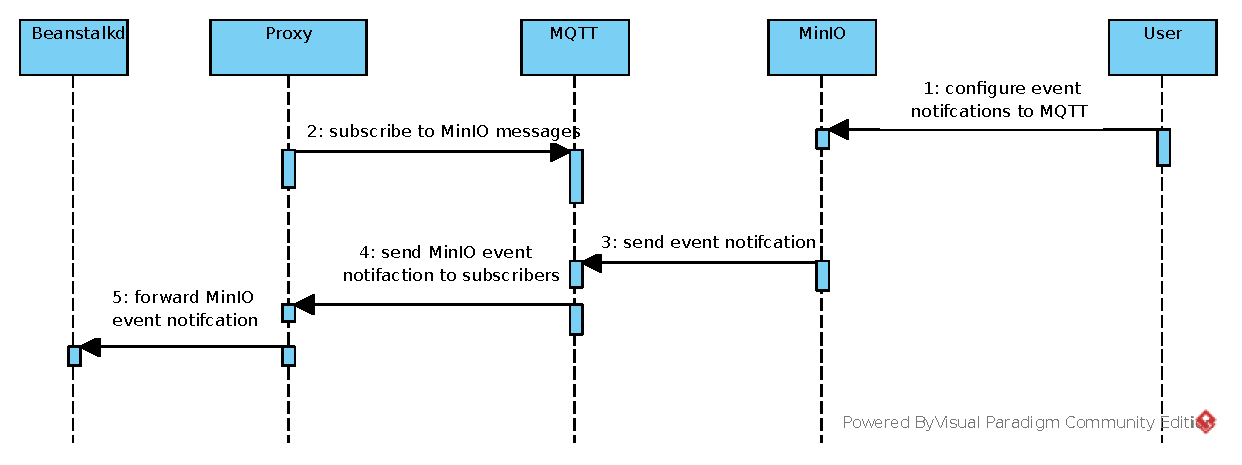
\includegraphics[angle=90,height=0.78\textheight]{obrazky-figures/minio-proxy.eps}
        %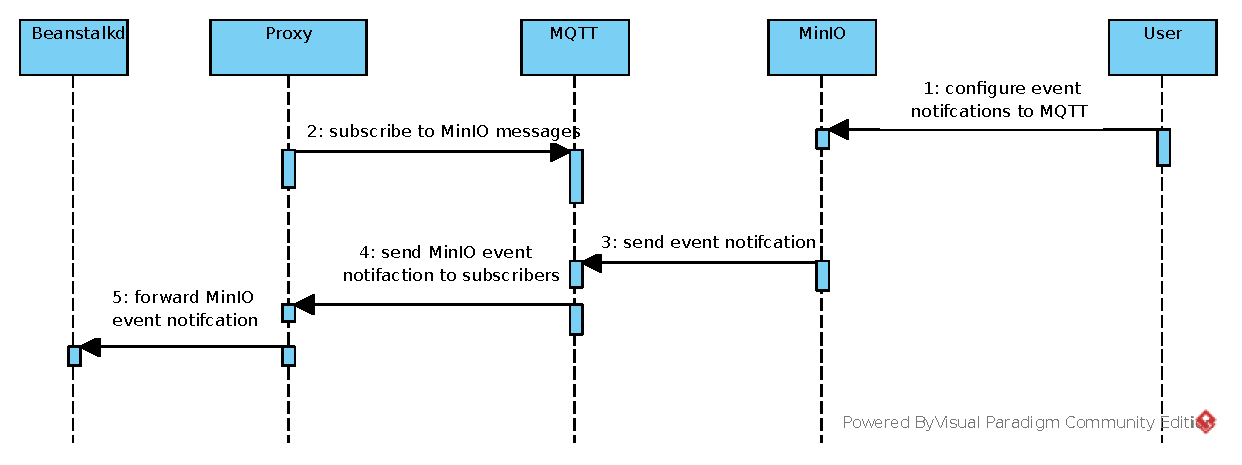
\includegraphics[width=1\textwidth]{obrazky-figures/minio-proxy.eps}
        \caption{Sequence diagram of proxy application allowing publishing events from MinIO to Beanstalkd.}
        \label{fig:minioProxy}
    \end{figure}

    Figure \ref{fig:minioProxy} shows a sequence diagram of the proposed proxy application for MQTT. The user configures MinIO event notifications using \textit{MinIO client} or \textit{MinIO SDKs}. Proxy application subscribes for MinIO messages in MQTT. Once event notification is sent from MinIO to MQTT, MQTT will send the event notification to subscribers, in this case Proxy application. Proxy application will receive a message containing an event notification from MinIO and forward it to Beanstalkd.


\chapter{Implementation, experiments and assessment}

\chapter{Conclusion}

%=========================================================================
